%!TEX root = jsba_main.tex
% Theoretical background 

\section{Theoretical Background}
\label{sec:theo}

In the following section there will be given an introduction to the distributed database terminology. The further sections give an overview of the 
architecture, fragmentation and replication that take place in such distributed systems as well as some advantages and disadvantages.
\todo[inline]{Query processing or own subsection?}

\subsection{Distributed Databases}
\label{sec:theo_ddb}

\subsubsection{Terminology}
\label{sec:theo_ddb_term}
A \emph{distributed database}~(DDB) can be defined as multiple, logically interconnected databases spread across a computer network~\cite[p.~4]{Ozsu1991}, such
that the physical presence of the data may be dispersed spatially instead of having one single database hoarding all the data at a certain location physically.
On top of this DDB, there is often a so-called \emph{distributed database management system}~(DDBMS) which manages the underlying databases and the access to 
the data, and the users are enabled to work with the data of the DDB without noticing the physically distribution, i.e. in a transparent 
manner~\cite[p.~4f.]{Ozsu1991}.
This results, from the point of view of a user, in a logically single database, which can be queried in the same way as a non-distributed database. 
Furthermore, users can benefit from a physical distribution of the data depending on an architectural design because they can communicate with the 
geographically closest site where one of the databases resides reducing the network communication delay, and concurrent access of the DDB can be handled in a 
distributed way, too, exploiting the fact that more servers imply more computing power for the \emph{distributed database system}~(DDBS). Additionally, a DDBS 
can provide an improved availability compared to a non-distributed database, e.g. when the data is replicated. This implies that the data can be reached from 
multiple sites even if there is a failure of one of the databases or of parts of the communication network. In this way, users will have a chance to be able
to still retrieve the data regardless of parts of the database being not available.


\subsubsection{Architecture}
\label{sec:theo_ddb_arch}
\defcitealias{Ignite}{Apache Ignite\texttrademark{}}
An architecture of a distributed database mangement system could look like depicted in Figure~\ref{fig:ddbs_arch}. Four different locations interconnected via
a communication network are each holding a database which is connected to a DBMS managing the underlying database. The locations can be local, e.g. four 
computers or servers in one room, or global, e.g. four servers at different cities where the company holding this DDBS resides. The type of a DDBMS can be
classified as \emph{homogenous} or \emph{heterogenous} where in a homogenous DDBS all participating sites share the same DBMS locally and in a heterogenous
DDBS the sites may have a different DBMS with probably different data models \cite[p.~607]{Ramakrish2000}. For example, if in Figure~\ref{fig:ddbs_arch} all
DBMSs (DBMS 1 -- DBMS 4) are the same DBMS, e.g. all are \citetalias{Ignite} nodes, then the distributed database system would be homogenous (cf. 
\cite[Fig.~2]{Jadhav2017}). If at least one of the locations is in control of a second DBMS, the DDBS would be homogenous, which is also called a 
\emph{multidatabase system}. However, the heterogenity of a DDBS introduces "a significant cost in terms of performance, software complexity, and
administration difficulty" \cite[p.~608, l.13--14]{Ramakrish2000} regarding the management of the distributed data.

\begin{figure}[h]
    \centering
    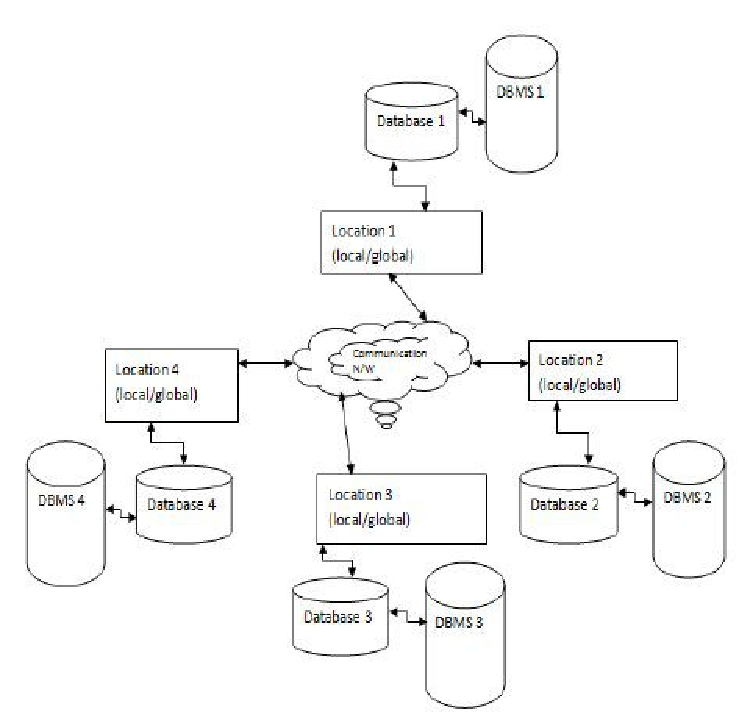
\includegraphics[width=0.8\textwidth,keepaspectratio=true]{img/DDBMS_Architecture.pdf}
    \caption{Architecture of a distributed database system from \cite[Fig.~1]{Kumar2013}}
    \label{fig:ddbs_arch}
\end{figure}

In \citet[p.~608f.]{Ramakrish2000} the three architecture approaches, \emph{Client-Server}, \emph{Collaborating Server} and \emph{Middleware}, are 
discussed. The first, really popular architectural model is characterized by a distinction between client and server processes resulting in a separation of
functionality, i.e. servers are responsible for data storage and management whereas clients provide user interfaces to query data from a server. In a
Colloborating Server system, in contrast, all servers are able to decompose received queries that concern data from multiple servers to subqueries. The
subqueries are then executed accordingly at the servers on their locally stored data and a result is computed from all the servers' answers. This is also
described in Section~\ref{...}. \todo[inline]{ref}
In Middleware systems the task of query management and decomposition is handled by a single server and all other servers only need to perform queries against
their local data.



\subsubsection{Fragmentation}
\label{sec:theo_ddb_frag}
The relations of distributed databases can be partitioned into fragments of the relations, i.e. the data from the tables is split up and assigned to one or 
more of the databases that belong to the DDBS. The amount of data per database can be reduced by doing so. This \emph{fragmentation} can be achieved by using
a certain fragmentation strategy and the resulting fragments, which contain parts of the whole data set, can then be dispersed across the network by mapping
the fragments to databases that possibly reside at different physical locations which are not necessarily geographically distant. The in the following 
introduced fragmentation alternatives will be elucidated by ways of small "toy" examples in Example~\ref{sec:theo_ddb_exmp}.

One strategy to obtain a fragmentation of the data is the so-called \emph{horizontal fragmentation} \cite[p.~105]{Ozsu1991} that divides a relation in a 
row-wise manner into smaller portions with only some of tuples that were contained in the original relation, i.e. a relation $R$ can be divided into fragments
$F_1, F_2,\dots, F_n$ by assigning each tuple $\mu$ of the relation $R$ to at least one fragment $F_i,~i\in\{1,\dots,n\}$. The result of this is that for all 
$i\in\{1,\dots,n\},~F_i \subseteq R$. Additionally, if there is no replication (cf. Section~\ref{sec:theo_ddb_repl}) applied to the data and each tuple is only
assigned to exactly one fragment, the fragments are pairwise disjoint ($\forall \mu \in F_i$ it holds that $\mu \notin F_j, i\neq j, i,j\in\{1,\dots,n\}$) 
if the relation $R$ does not contain any duplicate tuples itself. In the relational algebra such a \emph{primary horizontal fragmentation} can be described by
a selection operation on the relation $R$ \cite[p.~109]{Ozsu1991}, whereas the selection condition defines the wanted mapping of tuples to fragments. 
Regarding this primary horizontal fragmentation, a further fragmentation of another relation $S$ can be \emph{derived} by computing the semi-join of the
relation $S$ with fragments $F_i,~i\in\{1,\dots,n\}$ of the primary relation $R$ \cite[p.~116f.]{Ozsu1991}, i.e. the derived fragments $G_i$ of the relation
$S$ are computed as $G_i=S \ltimes F_i$ for $i\in\{1,\dots,n\}$. The \emph{derived horizontal fragmentation} depends on the underlying primary horizontal
fragmentation, and, to prevent tuples in $S$ from getting lost during the semi-join with fragments of $R$, it is necessary to have for each tuple $y\in S$ 
matching tuples in $R$ in order to let the tuples from $S$ "survive" the semi-join. An integrity constraint in form of a foreign key reference of the relation
$S$ to the relation $R$ can be used to enforce this condition for the sake of completeness of the derived fragmentation. Though with the definition of the 
derived horizontal fragmentation on a semi-join, inherently replication of tuples of $S$ in the derived fragments may occur if tuples in $S$ match multiple
tuples that belong to different fragments of $R$ \cite[p.~121]{Ozsu1991}. This causes the fragments $G_i$ of $S$ not to be disjoint in general which is equal
to a partial replication as described in Section~\ref{sec:theo_ddb_repl}.


On the other hand, a \emph{vertical fragmentation} \cite[p.~122]{Ozsu1991} is a columnwise division of a relation $R$, such that each of the resulting
fragments $F_1,F_2,\dots,F_n$ has a subset of the attributes of the relation $R$. To identify the original tuple to which a partitioned tuple of one of the
fragments belongs to, it is necessary to have a primary key defined on the relation $R$ which can be stored with the subset of attributes of the tuple that is
assigned to a fragment. If it is not the case that a primary key is set for the relation $R$, then an abstract, maybe randomly generated unique identifier has 
to be introduced, i.e. as additional attribute, in order to match tuple fragments to their source. 

Another fragmentation strategy, which will only be mentioned here and not further analyzed, is the so-called \emph{hybrid fragmentation} or 
\emph{nested fragmentation} \cite[p.~135f.]{Ozsu1991} that can be achieved by nesting horizontal and vertical fragmentations on a relation giving a complex
partitioning of the data and arising lots of issues to consider when implementing an application based on data that is fragmented by such type of fragmentation
strategy.

\begin{exmp} \label{sec:theo_ddb_exmp}
$ $\newline
    \begin{center}
    \begin{tabular}{c|c} 
         $a$ & $b$\\
         \hline
         0 & x \\
         1 & x \\
         2 & y \\
         3 & z \\
         7 & g \\
    \end{tabular}
    \captionof{table}{Relation $R$ with primary key $a$ and attribute $b$ (foreign key on $S.b$; see Table~\ref{tab:s})}
    \label{tab:r}
    \end{center}
$ $\newline
Consider having three fragments $F_1$, $F_2$ and $F_3$ of the relation $R$ which contains the tuples $\{(0,x), (1,x), (2,y), (3,z), (7,g)\}$ over the 
attributes $a$ and $b$, as shown in Table~\ref{tab:r}. 
A possible horizontal fragmentation is $F_1=\{(0,x), (1,x)\}$, $F_2=\{(2,y), (3,z)\}$ and $F_3=\{(7,g)\}$. 
This fragmentation is illustrated by Table~\ref{tab:r_frag} and could be obtained from the three selections $F_1=\sigma_{a \leq 1}(R)$,
$F_2=\sigma_{a \geq 2~\land~a \leq 5}(R)$ and $F_3=\sigma_{a \geq 6}(R)$. Here, each row of the table, i.e. each tuple $\mu \in R$, is assigned to exactly one
of the fragments $F_i,~i\in\{1,2,3\}$, so there is no duplication of any tuple and the fragments are pairwise disjoint, but each tuple $\mu \in R$ is somewhere
contained in one of the fragments. 
Hence, the union $F_1 \cup F_2 \cup F_3$ of all the fragments yields the original tuple set, which means that the partitioned relation $R$ can be reconstructed
from the fragments, because each of the original tuples is found in (at least) one fragment. Due to the fact that this primary horizontal fragmentation is
complete and disjoint and that the fragmentation can be reverted by reconstruction of the original relation, the three fragmentation correctness rules
\cite[p.~103]{Ozsu1991} are fulfilled.

\begin{table}[h]
    \hspace*{\fill}
    \begin{tabular}{c|c}
        $a$ & $b$\\
        \hline
        0 & x \\
        1 & x
    \end{tabular}
    \hfill
    \begin{tabular}{c|c}
        $a$ & $b$\\
        \hline
        2 & y \\
        3 & z
    \end{tabular}
    \hfill
    \begin{tabular}{c|c}
        $a$ & $b$\\
        \hline
        7 & g \\
         & 
    \end{tabular}
    \hspace*{\fill}
    \caption{Horizontal fragments $F_1$, $F_2$ and $F_3$ (from left to right)}
    \label{tab:r_frag}
\end{table}

According to this primary horizontal fragmentation of $R$, a derived horizontal fragmentation of $S=\{(x, 0.5), (y, 0.3), (g, 9.9)\}$ (Table~\ref{tab:s}) over 
the attributes $b$ and $c$ is obtained by computing the previously stated definition using a semi-join, fragment $G_i = S \ltimes F_i$ for $i\in\{1,2,3\}$.
Based on the matches of tuples from $S$ with tuples in the fragments $F_i$, the derived fragments are $G_1=\{(x,0.5)\}$, $G_2=\{(y, 0.3)\}$ and 
$G_3=\{(g, 9.9)\}$ (Table~\ref{tab:s}).


\begin{table}[h]
    \hspace*{\fill}
    \begin{center}
    \begin{tabular}{c|c}
        $b$ & $c$\\
        \hline
        x & 0.5 \\
        y & 0.3 \\
        g & 9.9
    \end{tabular}
    \hspace{20pt}
    \begin{tabular}{c|c}
        $b$ & $c$\\
        \hline
        x & 0.5
    \end{tabular}
    \hspace{5pt}
    \begin{tabular}{c|c}
        $b$ & $c$\\
        \hline
        y & 0.3
    \end{tabular}
    \hspace{5pt}
    \begin{tabular}{c|c}
        $b$ & $c$\\
        \hline
        g & 9.9
    \end{tabular}
    \caption{Relation $S$ with attributes $b$ and $c$ (leftmost), derived fragments $G_1$, $G_2$ and $G_3$}
    \label{tab:s}
    \end{center}
\end{table}

For the demonstration of an exemplary vertical fragmentation, consider the view $T$ calculated as the left outer join of the two relations $R$ and $S$, 
$T~=~R~{\tiny \textifsym{d|><|}}~S$ over the attribute set $\{a,b,c\}$. 
This left outer join yields the tuple set $\{(0,x,0.5), (1,x,0.5), (2,y,0.3), (3,z,null), (7,g,9.9))\}$ (Table~\ref{tab:join_vert_frag}). The so obtained
relation (or view) can be partitioned vertically based on the two attribute subsets $\{a,b\}$ and $\{b,c\}$ that produce two vertical fragments $H_1$ and 
$H_2$, which are also depicted in Table~\ref{tab:join_vert_frag} next to the original relation. Here, each tuple of one of the vertical fragments contains the
attribute a, which is, in this case, a unique identifier for the original tuple from $T$.

\begin{table}[h]
    \centering
    \begin{tabular}{c|c|c}
        $a$ & $b$ & $c$ \\
        \hline
        0 & x & 0.5 \\
        1 & x & 0.5 \\
        2 & y & 0.3 \\
        3 & z & null \\
        7 & g & 9.9 \\
    \end{tabular}
    \hspace{20pt}
    \begin{tabular}{c|c}
        $a$ & $b$ \\
        \hline
        0 & x \\
        1 & x \\
        2 & y \\
        3 & z \\
        7 & g \\
    \end{tabular}
    \hspace{5pt}
    \begin{tabular}{c|c}
        $a$ & $c$ \\
        \hline
        0 & 0.5 \\
        1 & 0.5 \\
        2 & 0.3 \\
        3 & null \\
        7 & 9.9 \\
    \end{tabular}
    \caption{$R~{\tiny \textifsym{d|><|}}~S$, vertical fragments $H_1$ and $H_2$}
    \label{tab:join_vert_frag}
\end{table}

\end{exmp}



\subsubsection{Replication}
\label{sec:theo_ddb_repl}
The \emph{data replication} as discussed in \citet{Wiese2014} is not relevant for the implementation part in this work, and so this topic will only be
mentioned here and the investigations on it will be kept short as it still is an important part of distributed databases. Replication is a design approach
for a DDBS that is used for storing the data together with copies of the data. The data is duplicated and can be distributed multiple times to even different
sites such that a the same data is present on different servers. In contrast to this, the data can also be \emph{partitioned} where none of the data fragments,
which are obtained from a fragmentation as analyzed in Section~\ref{sec:theo_ddb_frag}, is duplicated. There exist two alternative basic strategies for a 
replication design \cite[p.~12]{Ozsu1991}. One of them is the \emph{full replication} where the whole database is stored at each site, i.e. the data is
distributed to each server and so each server has exactly the same data set as all other servers. The other one is the \emph{partial replication} where each
of the data partitions can distributed to more than one server. A partial replication for example could be used in case of having each partition at a server 
that is primarily responsible for that partition (primary partition) and at some other servers where the partitions are held as backup copies for the primary
partition.
\todo[inline]{maybe refer to example ignite (picture)}


\subsubsection{Advantages and Disadvantages of DDBMS}
Using distributed databases for storing and managing information can be advantageous. As already mentioned, the distribution of the data across multiple 
servers can provide features like higher availability of the data, which can come from failure tolerance, as well as more efficient interaction with the DDBS. 
Several advantages of distributed database systems are (cf. \citep{Jadhav2017} and \cite[p.~8ff.]{Ozsu1991}):

\begin{enumerate}
    \item Local Autonomy: Data that is frequently accessed from a certain user group can be placed at the site which is the closest one to the user group
            allowing for local control and indepent access.
    \item Improved Performance: Parallelizing queries and resource usage can lead to higher efficiency.
    \item Improved Reliability/Availability: Distributed data has a higher resistance to inaccessibility in case of a failure because it may be retrieved from
            another site and work on at least the part of the data which is not affected by a failure can be guaranteed. 
    \item Expandability: The DDBS can be simply expanded by e.g. additional servers that improve the load balancing abilities of the system
    \item Shareability: Distributed databases inherently offer the possibility to share the stored data
\end{enumerate}

On the contrary, one big disadvantage of a DDBS is that installation, control and maintenance of such a system are really hard because of the way
more complex appearance of a DDBS compared to the centralized database concept \citep{Jadhav2017}. The design of a DDBS is also crucial as it can cause the 
system to be less efficient if the design is not well-suited to the application's requirements what can lead to bad resource usage and high communication 
costs in the interconnecting network. More issues are security of system and data, which demand some extra effort in terms of protection because the sites and 
data fragments are not centralized but remote making them more vulnerable if not secured accordingly, and economics where more infrastructure and hardware for 
a distribution to multiple sites come along with higher costs \cite{Kumar2013}.



\todo[inline]{Distributed query processing --> Öszu; Ramakrishnan p.614}